 \documentclass[book.tex]{subfiles}
\begin{document}


\section{Audio and Heartbeat} 
\label{audio_and_heartbeat}
The audio and heartbeat system runs concurrently with the rest of the program. On an operating system supporting neither multi-processes nor threads this means using interrupts to stop normal execution and perform tasks on the side.\\
\par
The idea is to configure the hardware to trigger a hardware interrupt at a regular interval. This interrupt is caught by a system called PIC which transforms it into a software interrupt, or IRQ. The software interrupt ID is used as an offset in a vector to look up a function belonging to the engine. At this point, the CPU is stopped (a.k.a: interrupted) from doing whatever it was doing (likely running the 2D renderer), and it starts running the interrupt handler which is called an ISR\footnote{Interrupt Service Routine}. We now have two systems running in parallel.\\
\par
\begin{figure}[H]
  \centering
  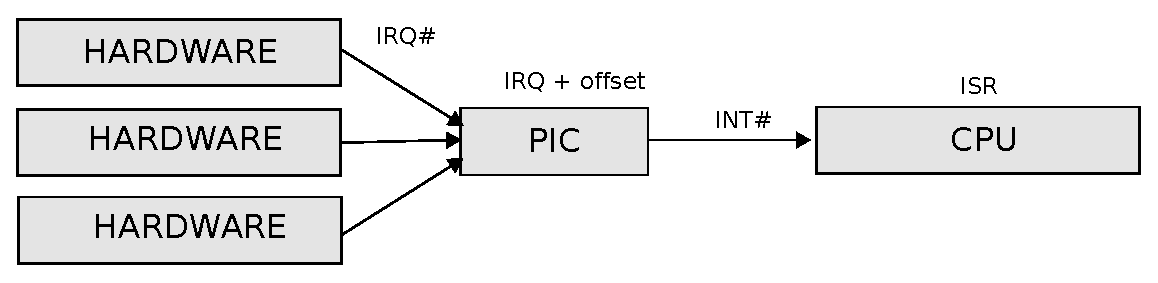
\includegraphics[width=\textwidth]{imgs/drawings/irqs/explanationsvg.eps}
  \caption{Hardware interrupts are translated to software interrupt via the PIC.}
\end{figure}
\par
 Since interrupts keep triggering constantly from various sources, an ISR must choose what should happen if an IRQ is raised while it is still running. There are two options.  The ISR can decide it needs a "long" time to run and disable other IRQs via the IMR \footnote{Interrupt Mask Register}. This path introduces the problem of discarding important information such as keyboard or mouse inputs.\\
 \par
 Alternately, the ISR can decide not to mask other IRQs and do what it is supposed to do as fast as possible so as to not delay the firing of other important interrupts that may lose data if they aren't serviced quickly enough. Keen Dreams uses the latter approach and keeps tasks in its ISR very small and short. 

\subsection{IRQs and ISRs}
The IRQ and ISR system relies on two chips: the Intel 8254 which is a PIT\footnote{Programmable Interval Timer} and the Intel 8259 which is a PIC\footnote{Programmable Interrupt Controller}. The PIT features a crystal oscillating in square waves. On each period, it decrements its three counters. Counter \#2 is connected to the buzzer and generates sounds. Counter \#1 is connected to the RAM in order to automatically perform something called "memory refresh"\footnote{Without frequent refresh, DRAM will lose its content. This is one of the reasons it is slower and SRAM is preferred in the caching system.}. Counter \#0 is connected to the PIC. 
When counter \#0 hits zero it generates an IRQ\footnote{Interrupt Request Line: Hardware lines over which devices can send interrupt signals to the CPU.} and sends it to the PIC.\\

\
\par
\begin{figure}[H]
  \centering
  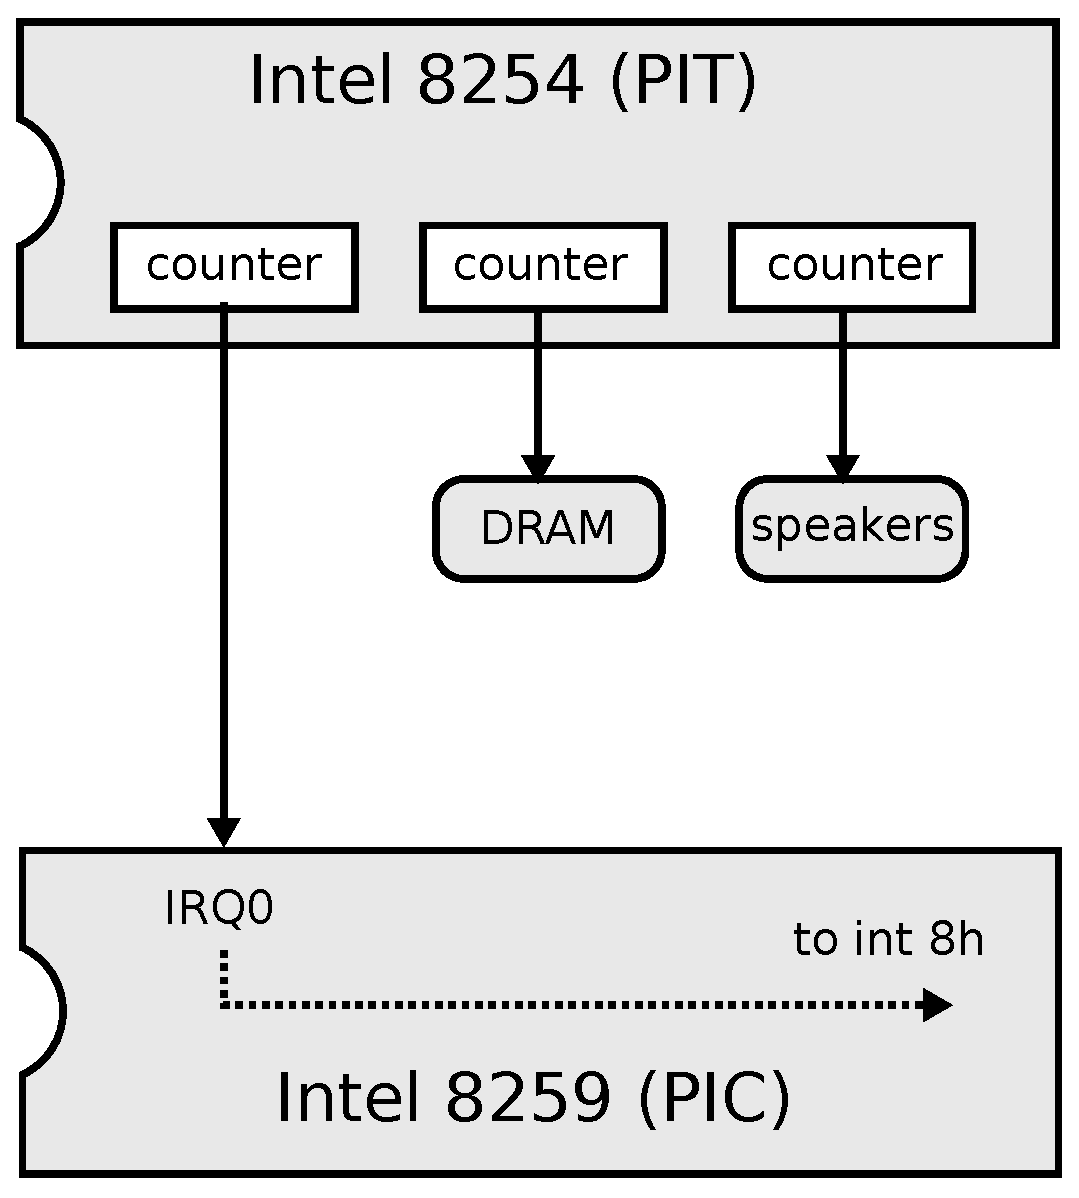
\includegraphics[width=.65\textwidth]{imgs/drawings/heatbeats.eps}
  \caption{Interactions between PIT and PIC.}
\end{figure}
\par

The PIC's hardware IRQ-0 to IRQ-8 are mapped to the Interrupt Vector starting at Offset 8 (resulting in mapping to software interrupts INT08 to INT0F). \pagebreak

\begin{figure}[H]
	\centering
	\begin{tabularx}{\textwidth}{ l p{.5\textwidth}  }
	  \toprule
	  \textbf{I.V.T Entry \#} & \textbf{Type} \\ \bottomrule

	  00h	&	CPU divide by zero \\
01h	&	Debug single step \\
02h	&	Non Maskable Interrupt \\
03h	&	Debug breakpoints \\
04h	&	Arithmetic overflow \\
05h	&	BIOS provided Print Screen routine \\
06h	&	Invalid opcode \\
07h	&	No math chip \\
08h & IRQ0, System timer \\
09h & IRQ1, Keyboard controller \\
0Ah & IRQ2, Bus cascade services for second 8259 \\
0Bh & IRQ3, Serial port COM2 \\ 
0Ch & IRQ4, Serial port COM1 \\
0Dh & IRQ5, LPT2, Parallel port (HDD on XT) \\
0Eh & IRQ6, Floppy Disk Controller \\
0Fh & IRQ7, LPT1, Parallel port \\
10h & Video services (VGA)\\
11h & Equipment check \\
12h & Memory size determination \\
		\bottomrule
	\end{tabularx}
	\caption{The Interrupt Vector Table (entries 0 to 18).}
\end{figure}
Notice \#8 which is associated with the System timer and usually updates the operating system clock at 18.2 ticks per second. Because IVT \#8 was hijacked, the operating system clock is not updated while Commander Keen runs. Upon exiting the game, DOS will run late by the amount of time played.\\
\par
Using these two chips and placing its own function at Interrupt Vector Table (IVT) \#8, the engine can stop its runtime at a regular interval, effectively implementing a subsystem running concurrently with everything else.\\
\par


\subsection{PIT and PIC}
The PIT chip runs at 1.193182 MHz. This initially seems like an odd choice from the hardware designers, but has a logical origin. In 1980 when the first IBM PC 5150 was designed, the common oscillator used in television circuitry was running at 14.31818 MHz. As it was mass produced, the TV oscillator was very cheap so utilizing it in the PC drove down cost. Engineers built the PC timer around it, dividing the frequency by 3 for the CPU (which is why the Intel ran at 4.7MHz), and dividing by 4 to 3.57MHz for the CGA video card. By logically ANDing these signals together, a frequency equivalent to the base frequency divided by 12 was created. This frequency is 1.1931816666 MHz. By 1991, oscillators were much cheaper and could have used any frequency but backward compatibility prevented this.\\

\subsection{Interrupt Frequency}
Each counter on the PIT chip is 16-bit, which is decremented after each period. An IRQ is generated and send to the PIC whenever the counter wraps around after 2\textsuperscript{16} = 65,536 decrements. So at default, the interrupts are generated at a frequency of 1.19318MHz / 65,536 = 18.2Hz. Some programs require a faster period than the 18.2 interrupts/second standard rate (for example, execution profilers). So they reprogram the timer by changing the counter value.\\
\par
\begin{minipage}{\textwidth}
\lstinputlisting[language=C,morekeywords={longword}]{code/set_timer.c}
\end{minipage}
\par
Note that \cw{SDL\_SetTimer0} is using a frequency of 1.192755MHz, instead of the PIT documented 1.193182MHz. Most likely at the time Keen Dreams was develop, the actual frequency of the PIT chip was not known by Jason Blochowiak and he derived the value based on the standard 18.2 interrupts per second * 65,536 = 1192755Hz.\\
\par
So the engine can decide at what frequency to be interrupted, depending on the type of sound/music it needs to play and what devices will be used. As a result, two frequencies are defined: 
\begin{enumerate}
\item Running at 140Hz to play sound effects and music on the PC beeper, AdLib and SoundBlaster.
\item Running at 700Hz to play sound effects and music on Disney Sound Source.
\end{enumerate}
\par
\begin{minipage}{\textwidth}
\lstinputlisting[language=C]{code/set_sound_mode.c}
\end{minipage}
\par












\subsection{Heartbeats}
Each time the interrupt system triggers, it runs another small (yet paramount) system before taking care of audio requests. The sole goal of this heartbeat system is to maintain a 32-bit variable: \cw{TimeCount}.\\
\par
\begin{minipage}{\textwidth}
\lstinputlisting[language=C,morekeywords={longword}]{code/timecount.c}
\end{minipage}
\par
It is updated at a rate of 70 units per seconds, to match the VGA update\footnote{EGA was updated at a rate of 60Hz. Some games, like Keen Dreams, are developed with VGA already in mind.} rate of 70Hz. These units are called "ticks". Depending on how fast the audio system runs (from 140Hz to 700Hz), it adjusts how frequent it should increase \cw{TimeCount} to keep the game rate at 70Hz.\\
\par
Every system in the engine uses this variable to pace itself. The renderer will not start rendering a frame until at least one tick has passed. The AI system expresses action duration in tick units. The input sampler checks for how long a key was pressed, and the list goes on. Everything interacting with human players uses \cw{TimeCount}.\\






\end{document}










